
%Whereas during training, we allow users to fail at task completion for improved learning, during assistance in tasks, such as activities of daily living (ADL), we may want to insist on task success, user safety, or both. In these situations, we can modify the proposed filter to actively provide assistance. Instead of using a null controller input as the alternative to user input, we can engage the controller and replace rejected actions with optimal control, calculated by an MPC. In the next two subsections, we provide simulation results that demonstrate system behavior when the MIG-based filter is employed in assistance mode.

Whereas during assistance, we prevent users from failing at a task, during training we may want to allow failure for improved learning. In these situations, we can use the proposed filter without actively providing assistance. Instead of using a calculated controller input as the alternative to user input, we can simply reject ``wrong" user actions and wait for the user to figure out the ``correct" next action. 

In the following chapter, we demonstrate results of a human subject study, where we compare learning of the cart-pendulum inversion task between a group training with feedback in the from of the filter-based shared control and a group training for an equivalent duration of time without feedback. Details of how the experiment was set up can be found in Section~\ref{section: human experiments} of Chapter~\ref{chapter: methods}.

\section{Training Effect}

\begin{figure}[!h]
	\begin{center}
		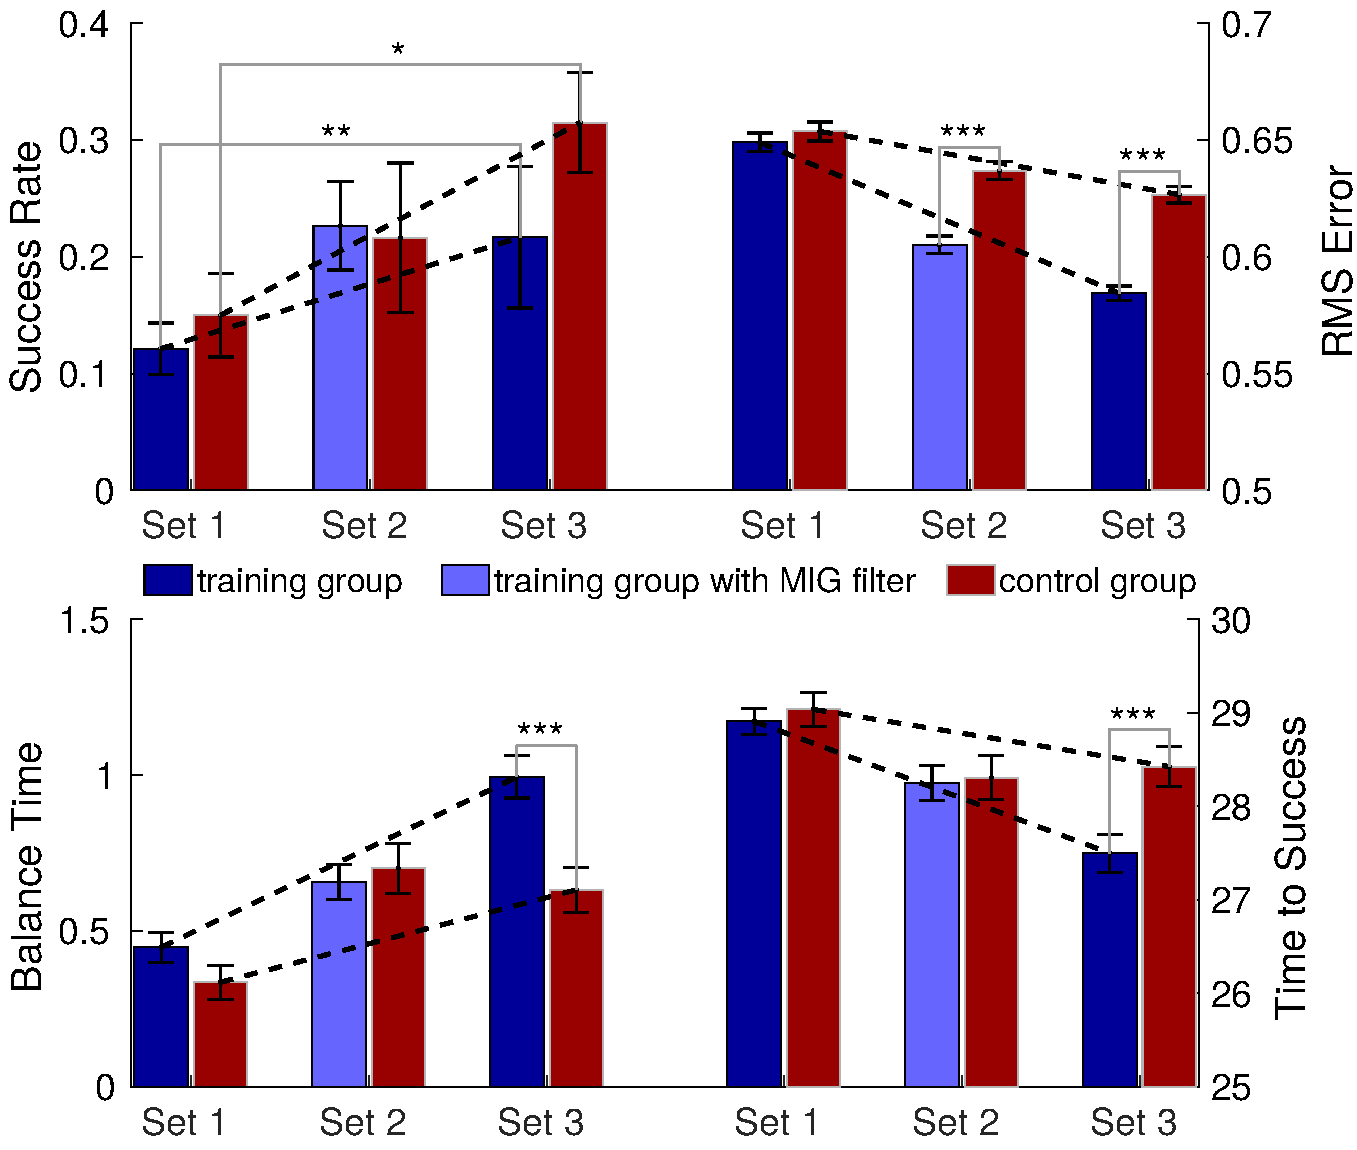
\includegraphics[width=\columnwidth]{training.pdf}
	\end{center}
	\caption{There was a training effect from training with the filter-based feedback compared to training with no feedback. The RMS error, balance time, and time to success of the training group in the final set was significantly better than that of the control group. It is also worth noting that as expected, pairwise comparisons of the two groups in set 1 show that there was not a significant difference in their baseline performance measurements. Moreover, set was consistently the most significant factor in performance improvements from set 1 to set 3, showing that both groups (training and control) improved significantly over time. Finally note that error bars indicate standard error and significance is indicated by $^*p<0.05$, $^{**}p<0.01$, $^{***}p<0.001$.}
	\label{fig: training}
\end{figure}

The main result we were looking for in the study was whether providing filter-based feedback through forceful interaction would improve learning. And indeed, we observed a significant training effect from training with filter-based feedback compared to training with no feedback for an equivalent duration of time, as visible in Fig.~\ref{fig: training}. \textit{Post hoc} analysis confirmed that both groups started the experiment at comparable skill levels and although training time was the main factor impacting improvement in performance (both groups improved over time), the training group improved significantly more than the control. Detailed statistical analysis is described below. 

A two-factor repeated measures ANOVA was used to assess the effects of the group (between-subjects) and set (within-subjects) on all performance measures listed in Section~\ref{metrics} of Chapter~\ref{chapter: methods}. The training group and control group were evaluated based on set 1 and set 3 only. Set 2 was left out of the ANOVA, so that effects of the assistance itself would not be measured in the analysis. Additionaly, pairwise comparisons were made between set 1 for both groups, between set 3 for both groups, and between set 1 and set 3 within each group using a paired 2 sample t-test. 

Firstly, we confirmed that there was on average no difference in skill at the onset of the experiment. Pairwise comparisons within each of the four measures (success rate, RMS error, balance time, and time to success) showed that in set 1 there was not a significant difference between the training group and control group. For instance, the main effect of group in set 1 on the RMS error was not significant ($F(1,26)=1.615, p = 0.215$)---there was not a significant difference between the training group ($mean =0.612, SD =0.088$) and the control group ($mean = 0.639 , SD=0.067$) in set 1. The same was true for the three other metrics. According to 2-sample t-tests, the differences between the two groups were also not significant across all 4 metrics ($p>0.01$).

Secondly, we found that time had the most significant impact on learning. The factorial ANOVA revealed that for success rate the main effect of set yielded an F ratio of $F(1,50)=7.555,\ p=0.008$, meaning that users were more successful in set 3 ($mean =0.280 , SD = 0.223$) than in set 1 ($mean = 0.140,\ SD = 0.100$) regardless of the type of practice in set 2. Similarily, the RMS error showed that the main effect of set yielded an F ratio of $F(1,26) = 41.551, p<0.001$, indicating a significant difference between set 1 ($mean =0.651, SD =0.085$) and set 3 ($mean =0.599, SD =0.072$). The main effect for set on the balance time yielded an F ratio of $F(1,26)=15.328,\ p<0.001$, indicating a significant difference between the balance time in set 1 ($mean = 0.408, SD = 1.053$) and set 3 ($mean = 0.866, SD = 1.476$). The main effect of set on time to success was also significant ($F(1,26)=18.992,\ p<0.001$), with set 3 ($mean = 27.830, SD = 4.433$) outperforming set 1 ($mean = 28.955,SD =3.175$). Set had a significant effect on increases across all metrics, indicating that participants were continuously improving with time regardless of the feedback that was provided. 

Thirdly, we observed that there was more improvement among members of the training group than control. When training group and control group were compared in set 3 using 2-sample t-tests, the training group performed better. The set 3 balance time of the control group ($mean =0.632, SD = 1.261$) was significantly less ($t(728)=3.643,p<0.001$) than the balance time of the training group ($mean = 0.994 , SD = 1.568$). The time to success was also significantly better ($t(738)=3.110, p=0.002$) in set 3 of the training group ($mean = 27.500, SD = 4.744$) compared to set 3 of the control group ($mean =28.43, SD = 3.74$). The same was true for the RMS error ($t(699)=-8.919,p<0.001$)---the RMS error of the training group in set 3 ($mean = 0.58, SD = 0.003$) was lower than the RMS error of the control ($mean = 0.63, SD = 0.004$). The RMS error, balance time, and time to success of the training group in the final set was significantly better than that of the control, while the difference for success rate was not statistically significant. 

Moreover, the RMS error showed that there was a significant interaction effect between group and set ($F(1,26)=5.099, p=0.0326$). This is indicated in Fig.~\ref{fig: training} by the two groups having similar means in set 1 but significantly different means in set 3, implying that the training had a greater impact on set 3 performance than the unassisted practice of the control group. For the other measures, the interaction effects were statistically insignificant---there was no significant interaction effect of group and set on balance time ($F(1,26)=1.048,\ p=0.315$), time to success ($F(1,26)=1.512,\ p=0.22983$) or success rate ($F(1,50)=0.111,\ p=0.740$). There was also no signifcant effect of group on any of the metrics: success rate ($F(1,50)=0.981,\ p=0.327$), balance time ($F(1,26)=1.562,\ p=0.223$), time to success ($F(1,26) = 1.114,\ p=0.301$), or RMS error ($F(1,26) = 1.824 ,\ p=0.189$). In summary, although there was not a significant effect of group on any of the  metrics, the RMS  error  showed  that there  was  a  significant  interaction  effect between  group  and set.  

% Although the change in success rate from set 1 to set 3 was significant for both the control group ($t(9)=3.152,\ p = 0.012$) and the experimental group ($t(17)=3.127,\ p=0.006$), the effect size of the training group ($d=0.94$) from set 1 to set 3 was larger than the effect size of the control group ($d=0.77$). (XXX why report this only for success rate?) 

 % Note that the control group continued to improve their success rate with each set, possibly because their interaction with the robot did not change between sets as it did for the training group. 


\begin{figure}[!h]
	\begin{center} 
	\begin{multicols}{2}
		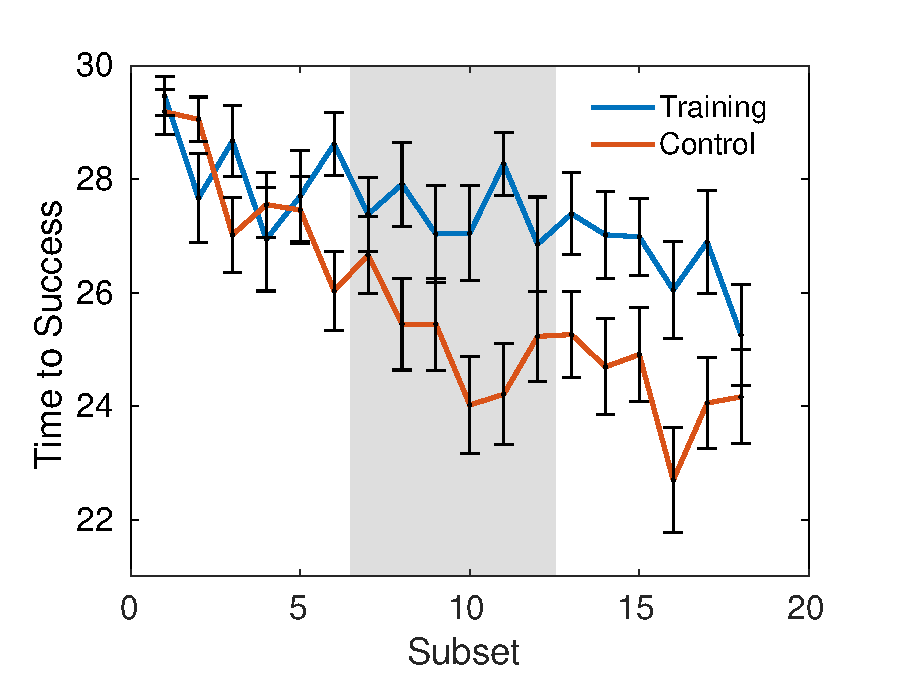
\includegraphics[width=0.85\columnwidth]{tts_plateau.eps}
		\caption*{}
		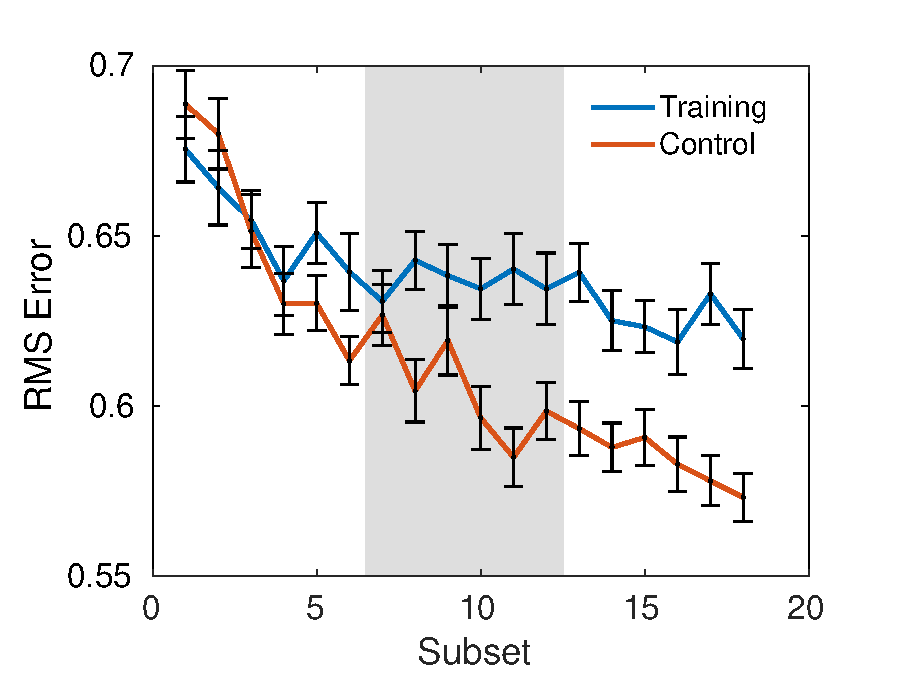
\includegraphics[width=0.9\columnwidth]{err_plateau.eps}
		\caption*{}
	\end{multicols}
	\end{center}
	\vspace{-1.2cm}
	\caption{Grey band covers subsets included in set 2 (the set, where the training group received feedback). Note that training and control groups showed similar improvement during set 1, while the training group showed faster improvement during set 2. Particularly with respect to the RMS error, the control group's improvement slows down drastically during set 2, while the training group keeps improving.}
	\label{fig: plateau}
\end{figure}


Finally, in order to assess how subject performance evolved over time, the baseline and post-training sets were analyzed using subsets containing five individual trials, rather than the sets of thirty trials used for the analysis above. As such, there were 6 subsets in each set as shown in Fig.~\ref{fig: plateau}. We can see that the training and control groups diverage in performance during the subsets of set 2. Particularly with respect to the RMS error, the control group plateaus in improvement while the training group keeps improving. These results support the hypothesis that subjects experience accelerated learning while receiving feedback through filter-based forceful interaction. 

 
\section{Real-Time Performance Improvement}

Like detailed in the section above, the two experimental groups performed similarly in their baseline trials. However, in set 2, the group using the filter outperformed the control group in terms of time to success, RMS error, and balance time.

The experimental group ($mean = 25.168, SD = 7.686$) had a lower time to success ($t(798.03) = -4.999, p = 7.067 \times {10}^{-7} $) than the control group ($mean = 27.418, SD = 5.266$). The RMS error of the experimental group ($mean = 0.605, SD = 0.087$) was also significantly lower ($t(753.59) = -5.925, p = 4.738 \times {10}^{-9} $) than that of the control group ($mean = 0.636, SD = 0.066$). Finally, the balance time of the experimental group ($mean = 2.358, SD = 3.469$) was higher ($t(691.51) = 7.28, p = 9.1 \times {10}^{-13}$) than that of the control group ($mean = 1.026, SD = 1.418$), showing that the filter was able to effectively assist subjects in the task and improve all task-specific metrics. There was no significant difference between the success rate of the control group and the experimental group during set 2 ($p = 0.335$), which makes sense because success rate can only be calculated per set rather than per trial and hence many less samples are available. Comparisons between the control and experimental groups are shown in Fig.~\ref{fig: training}. Overall, these results demonstrate that the MIG filter meets the commonly reported requirement of shared control schemes in that it assists subjects with the task while in use. 
 
 
\section{Features of Assist-As-Needed}
\label{skill correlation}

Like described in the Introduction in Chapter~\ref{chapter: intro}, studies emphasize the need for training interfaces to be assist-as-needed. This real-time adjustment to user performance is critical due to two factors:
\begin{enumerate}
\item users start at different skill levels requiring different levels of feedback and assistance
\item users exhibit varying performance levels over time because of either overall improvement at the task or temporary distractions and fatigue again requiring adequately adjusting levels of shared control.
\end{enumerate}
By remaining sensitive to user skill and current performance, the interface avoids overreliance on the assistance and encourages learning. Uniquely in comparsion to most available solutions, it adjusts its engagement on an instantenous basis without the need to specify or approximate additional parameters, such as machine trust in the user. In the sections below, we report experimental results that demononstrate correlations between controller engagement and both initial skill level and within-trial performance.


\subsection{Correlation with Initial Skill Level}

From the experimental results, a relationship was observed between participant skill level---estimated based on performance in unassisted trials---and the frequency of controller intervention in the training set. In this case, we calculate the success rate of the 30 trials from set 1 to approximate user skill level. We then use percent of rejected actions (PRA) values from individual trials in set 2 from the same users to identify the correlation---a scatter plot with the results is visible in Fig.~\ref{fig: MDA_corr_dotproduct}. A Pearson product-moment correlation coefficient was computed and a low negative correlation ($r=-0.14$, confidence interval $(-0.22)-(-0.06)$, $p=0.001$) was identified between overall success rate in set 1 and PRA in individual trials of set 2 for the training group ($n=18$). Similar but weaker correlations were identified between controller intervention and other task-specific metrics, such as balance time ($r=-0.09$, confidence interval $(-0.17)-(-0.007 )$, $p=0.03$) and time to success ($r=0.11$, confidence interval $0.086-0.25$, $p=0.01$).

Since subjects showed significant improvement during set 1 while getting used to the task and testing platform, we ran the same statistics using only the last 10 trials of set 1 to estimate participant skill level. Again, a Pearson product-moment correlation coefficient was computed and a low negative correlation ($r=-0.23$, confidence interval $(-0.31)-(-0.14)$, $p=1.0\times 10^{-7}$) was identified between overall success rate in the last 10 trails of set 1 and PRA in individual trials of set 2. Similar correlations were identified between controller intervention and other task-specific metrics, such as balance time ($r=-0.14$, confidence interval $(-0.23)-(-0.06)$, $p=0.0007$) and time to success ($r=0.24$, confidence interval $0.16-0.32$, $p=1.2\times 10^{-8}$).


\begin{table}[!h]
\begin{tabular}{c|c|c|c}
\textbf{Measure} & Test Sign & $\mathbf{r}$ & $p$ \\
\hline \hline
Success Rate & $-$& $\mathbf{-0.23}$ &  $1.0\times 10^{-7}$ \\
Balance Time & $-$& $\mathbf{-0.14}$ & $0.0007$ \\
Time to Success & $+$ & $\mathbf{+0.24}$ & $1.2\times 10^{-8}$ \\
%Error & $+$ & $\mathbf{-0.007}$ & $0.86$ \\
\end{tabular}
\vspace{0.7cm}
\caption{Correlation results between initial skill level and controller engagement. Pearson's correlation tests were performed by applying a linear model to the participant skill level, as estimated from performance measures in the last 10 trials of set 1, and the frequency of controller intervention in the training set---the PRA in set 2. The expected sign of the correlation coefficient ($r$) for a shared control scheme that is sensitive to the performance of the user is indicated in the column on the left. There was a weak but significant correlation between the current performance of the user and PRA for success rate, balance time, and time to success. For RMS error, results were statistically insignificant ($p=0.86$). }
\label{tab: initial skill}
\end{table}

\begin{figure}[!h]
	\begin{center}
		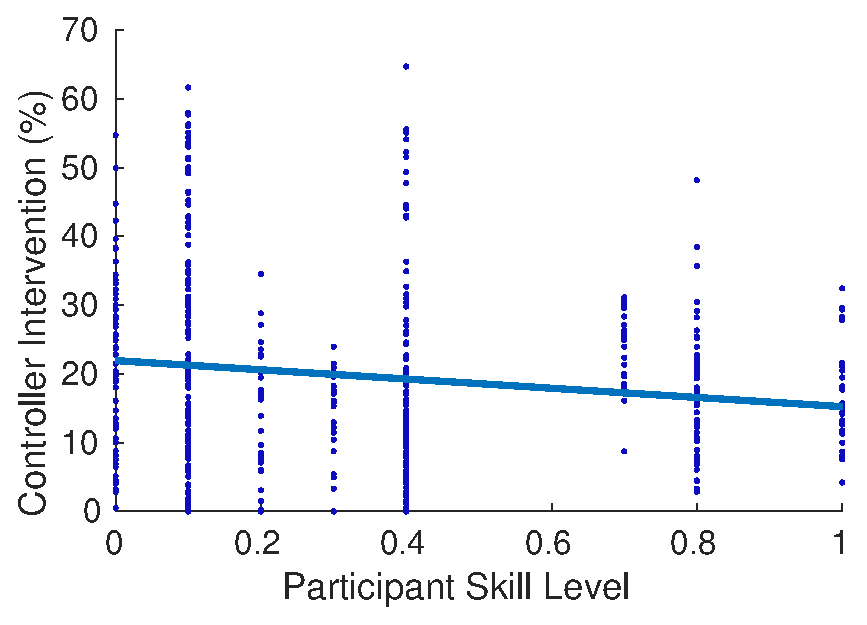
\includegraphics[width=0.8\columnwidth, keepaspectratio]{corr_plot_SKILLvsPAA.eps}\par
	\end{center}
	\caption{A correlation coefficient of $-0.23$ is observed between the success rate of the users in set 1 with no assistance and the rejection rate of the users' inputs in set 2 with assistance, suggesting a correlation between the users' adeptness at the task and the controller's intervention rate during assistance. }
	\label{fig: MDA_corr_dotproduct}
\end{figure}

Overall, for an experimental group of 18 participants, we obtained low but significant correlations \cite{cohen_statistics} between independently measured performance metrics and rejection rate (PRA) in assisted trials, suggesting a relationship between the users' skill level and the MIG filter's rate of intervention. Because the correlations are weak, additional subjects and analysis of other tasks are needed before the skill sensitivity is conclusive. However, our initial findings suggest that a MIG-based filter is a skill-sensitive paradigm that can be used for shared control. MIG-based feedback resembles assist-as-needed shared control schemes, which have been in previous studies shown to be advantageous for learning. 


\subsection{Correlation with User Performance}

Since the filter adjusts on an instaneous basis, we also looked at how it would adapt to a user's overall performance during engagement. We found a weak correlation ($r=0.17$) between the success rate and percent of rejected actions, which demonstrate that the controller engages less often when the user is performing better at the task. Correlation coefficients for other metrics were statistically insignificant, so more testing would have to be conducted to further evaluate the filter. 

Overall though, these results suggest that the proposed filter exhibits features of assist-as-needed paradigms both in terms of adaptation to initial user skill level and adaptation to real-time performance. 
